\begin{figure}[H]
    \centering
    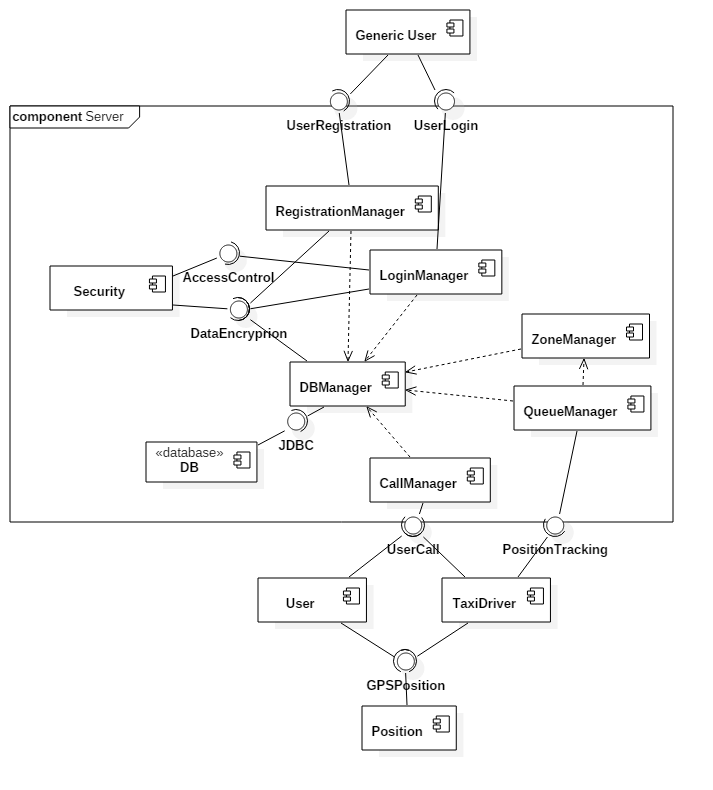
\includegraphics[width=14cm]{./Images/ComponentDiagram.png}
    \caption{Component diagram of our system}
    \label{fig:component-diagram}
\end{figure}


\subparagraph{Registration Manager}
This component handles the registration of a new user into the system, using some interfaces offered by the Security component.

\subparagraph{Login Manager}
This component handles the login of a user into the system, using some interfaces offered by the Security component.

\subparagraph{Database Manager}
This component manages the interaction with the database providing all the information asked by all the other components.

\subparagraph{Zone Manager}
This component coordinates all the zones the city is divided in.
\begin{itemize}
    \item It create the queues of every zone.
    \item When a taxi driver leaves a zone, the taxi driver must be removed from the previous queue in which he was, so the ZoneManager notifies the QueueManager, telling him the new zone of the taxi and the associated queue.
\end{itemize}

\subparagraph{Queue Manager}
This component manages the taxi drivers in a certain zone.
\begin{itemize}
    \item Add/delete a taxi driver from the queue
    \item Change the position of taxi drivers in the queues.
    \item When a request is incoming it searches for the right taxi driver to send the request to.
\end{itemize}

\subparagraph{Call Manager}
This component manages all the incoming/waiting calls for a taxi.
\begin{itemize}
    \item Retrieves all the information regarding the call.
    \item Updates the information of the calls when their status is changed.
\end{itemize}

\subparagraph{Position}
The scope of this component is to get the GPS positions of the devices that use it. Those components after using it send the data to the various components in the system. In particular The Taxi Driver component uses the data got by the Position component to track his position sending the information to the Queue Manager.

\subparagraph{Security}
This component offers some interfaces to grant security to the whole system.
For example  it prevent a user to have multiple login session on different devices at the same time.
